% !TeX TXS-program:compile = txs:///pdflatex/[--shell-escape]

\documentclass[11pt, letterpaper]{article}

\usepackage[utf8]{inputenc}
\usepackage{minted}
\usepackage[T1]{fontenc}
\usepackage{lmodern}
\usepackage{graphicx}
\usepackage{longtable}
\usepackage{wrapfig}
\usepackage{rotating}
\usepackage{amsmath}
\usepackage{textcomp}
\usepackage{amssymb}
\usepackage{hyperref}
\usepackage[spanish]{babel}
\usepackage[round]{natbib}
\usepackage{subcaption}

\title{\bfseries Tarea}
\author{Ángel García Báez}
\date{\today}
\setcounter{tocdepth}{4} 

\begin{document}
	
	% Página de presentación
	\begin{titlepage}
		\centering
		
\includegraphics[width=0.2\textwidth]{logo.png}\par
		\vspace{1cm}
		{\LARGE \bfseries Universidad Veracruzana \par}
		\vspace{1cm}
		{\Large Maestría en Inteligencia Artificial\par}
		\vspace{3cm}
		{\LARGE \bfseries Lógica difusa \par}
		\vspace{1cm}
		{\Large \bfseries Tarea 7. Modelando una función sen(x) con lógica difusa usando el método de Sugeno con Fuzzy Toolbox y en código matlab. \par}
		\vfill
		{\Large \textit{Ángel García Báez}\par}
		\vfill
		{\Large Dr. Sergio Hernández Méndez \par}
		\vfill
		{\Large \today \par}
	\end{titlepage}
	
	% Página exclusiva para la tabla de contenidos
	\newpage
	\tableofcontents
	\newpage
	
% Explicación breve

\section{Introducción}

En el presente reporte se plantea el problema de modelar o aproximar una función $sen(x)$ en el rango de $(0,2\pi)$ con lógica difusa y usando el método de Sugeno. Para ello, se tomo de base la función $sen(x)$ y se dividió en 9 tramos que posteriormente pasaron a ser las funciones de membresia de la variable de entrada y que mapean a la variable de salida.
Se hizo la implementación mediante el fuzzytoolbox de y se programo paso a paso.

Se muestra la comparativa de los resultados obtenidos tanto con el fuzzy toolbox como con el código hecho en matlab paso a paso para 3 escenarios distintos:

Cuando la variable de entrada es mínima, cuando es media y cuando es máxima.

\newpage


\section{Problema 1: Aproximación del $sen(x)$}

\subsection{Explicación del Problema}

Se quiere aproximar el comportamiento de la función $sen(x)$ en el rango de $(0,2\pi)$ haciendo uso de un sistema de lógica difusa con el método de Sugeno. Para ello unicamente se toma una variable de entrada X que tiene el rango ya mencionado.

La propuesta es dividir en 9 tramos el comportamiento de la función seno para generar 9 funciones de membresia triangulares en $X$. 


\subsection{Variables y sus codificaciones}

A continuación se listan los valores de las variables lingüísticas que se propusieron para el Ángulo (X) y la salida del seno(x) como sigue:


\begin{enumerate}
	
	 \item Ángulo (x) con función triangular: 
	
	\item R1 $[-1.5708, 0, 1.5708]$, 
	\item R2 $[0, 0.7854, 1.5708]$ 
	\item R3 $[0.7854, 1.5708, 2.3562]$
	\item R4 $[1.5708, 2.3562, 3.1416]$
	\item R5 $[2.3562, 3.1416, 3.9270]$
	\item R6 $[3.1416, 3.9270, 4.7124]$
	\item R7 $[3.9270, 4.7124, 5.4978]$
	\item R8 $[4.7124, 5.4978, 6.2832]$
	\item R9 $[5.4978, 6.2832, 7.8540]$.

	\begin{figure}[h]
		\centering
		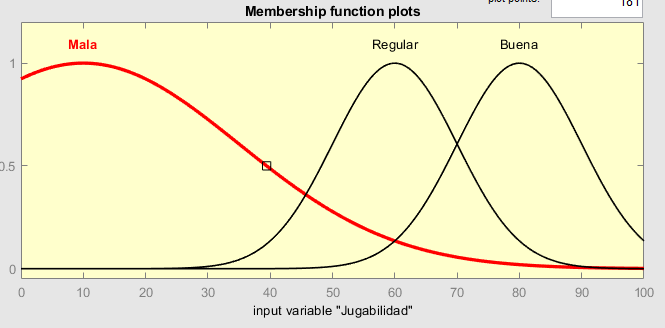
\includegraphics[width=0.8\textwidth]{IMG/P11.png}
		\caption{Funciones de pertenencia triangulares para la variable de entrada Ángulo (x)}
	\end{figure}

	\newpage

	 Valor del seno (sinx): 
	\item O1 (valor constante de 0), 
	\item O2 (valor constante de 0.7071),
	\item O3 (valor constante de 1), 
	\item O4 (valor constante de 0.7071), 
	\item O5 (valor constante de 0), 
	\item O6 (valor constante de -0.7071), 
	\item O7 (valor constante de -1), 
	\item O8 (valor constante de -0.7071) y 
	\item O9 (valor constante de 0).
	\begin{figure}[h]
		\centering
		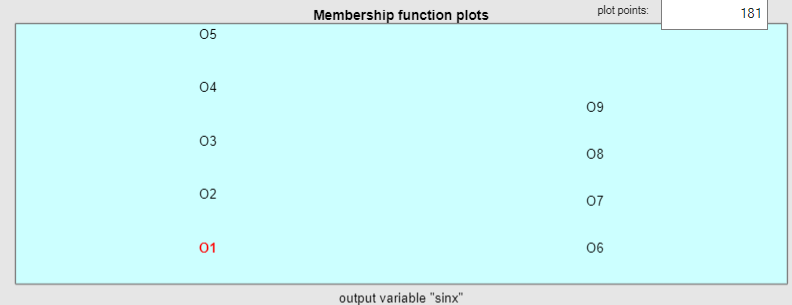
\includegraphics[width=0.8\textwidth]{IMG/P12.png}
		\caption{Valores constantes para la variable de salida seno(x) (método Sugeno)}
	\end{figure}
\end{enumerate}



\newpage 

Las funciones de membresia del Ángulo fueron modeladas con funciones triangulares, mientras que la salida del $seno(x)$ fue modelada con singletons (una triangular modificada en 1 solo valor) para mantener el sistema $sencillo$ y por su naturaleza discreta. \\

Se aplico el método de Sugeno para el procesado de las variables de entrada. 

\newpage

\subsection{Reglas de inferencia.}

A continuación se muestran las doce reglas que se construyeron para este problema:

\begin{enumerate}
	\item Si \textbf{X} pertenece a la región asociada a \textbf{R1}, entonces la \textbf{salida} es \textbf{\textit{0}}.
	\item Si \textbf{X} pertenece a la región asociada a \textbf{R2}, entonces la \textbf{salida} es \textbf{\textit{0.7071}}.
	\item Si \textbf{X} pertenece a la región asociada a \textbf{R3}, entonces la \textbf{salida} es \textbf{\textit{1}}.
	\item Si \textbf{X} pertenece a la región asociada a \textbf{R4}, entonces la \textbf{salida} es \textbf{\textit{0.7071}}.
	\item Si \textbf{X} pertenece a la región asociada a \textbf{R5}, entonces la \textbf{salida} es \textbf{\textit{0}}.
	\item Si \textbf{X} pertenece a la región asociada a \textbf{R6}, entonces la \textbf{salida} es \textbf{\textit{-0.7071}}.
	\item Si \textbf{X} pertenece a la región asociada a \textbf{R7}, entonces la \textbf{salida} es \textbf{\textit{-1}}.
	\item Si \textbf{X} pertenece a la región asociada a \textbf{R8}, entonces la \textbf{salida} es \textbf{\textit{-0.7071}}.
	\item Si \textbf{X} pertenece a la región asociada a \textbf{R9}, entonces la \textbf{salida} es \textbf{\textit{0}}.
\end{enumerate}
\newpage

\subsection{Gráficos del problema del problema}

La gráfica de superficie resultante de todo lo descrito previamente, es la siguiente:

\begin{figure}[h]
	\centering
	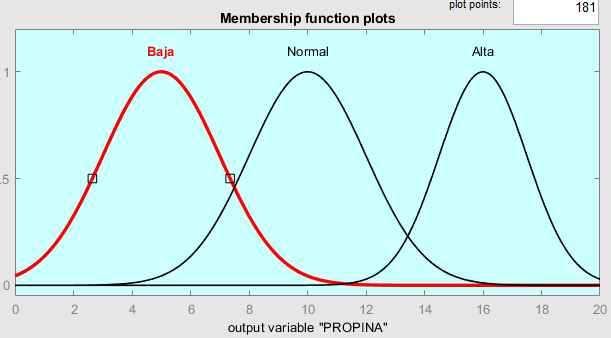
\includegraphics[width=1\textwidth]{IMG/P13.png}
\end{figure}

La gráfica resultante es un gráfico en 2 dimensiones que simula bastante bien el comportamiento del seno.

\newpage

\subsection{Implementación del problema del mesero paso a paso}

A continuación se explica como se implemento el sistema difuso para aproximar el seno paso a paso en matlab.

El primer paso fue identificar las variables de discurso: Ángulo (X) y la salida del $seno(x)$ en 0.\\

Con referencia a lo explicado en el libro de \cite{Cisneros2004}, se implemento la función de membresía tiangular tal y como la define a continuación:

$$
\mu_A(x) = 
\begin{cases}
	0, & x \le a \\
	\frac{x - a}{b - a}, & a < x \le b \\
	\frac{c - x}{c - b}, & b < x \le c \\
	0, & x > c
\end{cases}
$$


Posteriormente, se definieron los rangos de cada una de las funciones de membresía, dado que solo se usan funciones triangulares y singletons, se dejaron los rangos tal cual se había presentado anteriormente

Siguiendo con el proceso, fueron implementadas cada una las 9 reglas que ya se mostraron previamente y utilizando los resultados de las funciones de membresía como se describe a continuación:

El valor de activación de la regla:

$$
w_i = \mu_{A_i}(x_1) \cdot \mu_{B_i}(x_2)
$$

La contribución de la regla de salida:

$$
contribucion_i = w_i \cdot z_i
$$

\newpage

Por ultimo, ya que se contaban con las funciones de membresía y el sistema de reglas, dado que se van a trabajar con salidas singleton, la forma de deffuzificar las entradas para generar las salidas es mediante el método del promedio ponderado:


$$
z = \frac{\sum_{i=1}^{N} w_i \cdot z_i}{\sum_{i=1}^{N} w_i}
$$


donde:

\begin{itemize}
	\item \( x_i \) son los valores discretos de la variable de salida.
	\item \( \mu(x_i) \) es el grado de pertenencia de \( x_i \) en la función de pertenencia de la salida difusa.
	\item \( n \) es el número total de puntos discretos en el dominio de salida.
\end{itemize}

Una vez que el sistema esta listo y programado, se procede a hacer la comparativa con el toolbox de matlab.

\newpage

\subsection{Comparativa para la aproximación del seno}

A continuación se presentan los resultados que da el sistema programado paso a paso en matlab contra el resultado para el mismo sistema por parte del fuzzy toolbox en 3 escenarios distintos.

\subsubsection{Caso mínimo}

Para el caso mínimo, se propone un valor de $X = 0$.

\begin{figure}[h]
	\centering
	\begin{subfigure}{0.45\textwidth} % Reducido de 0.45
		\centering
		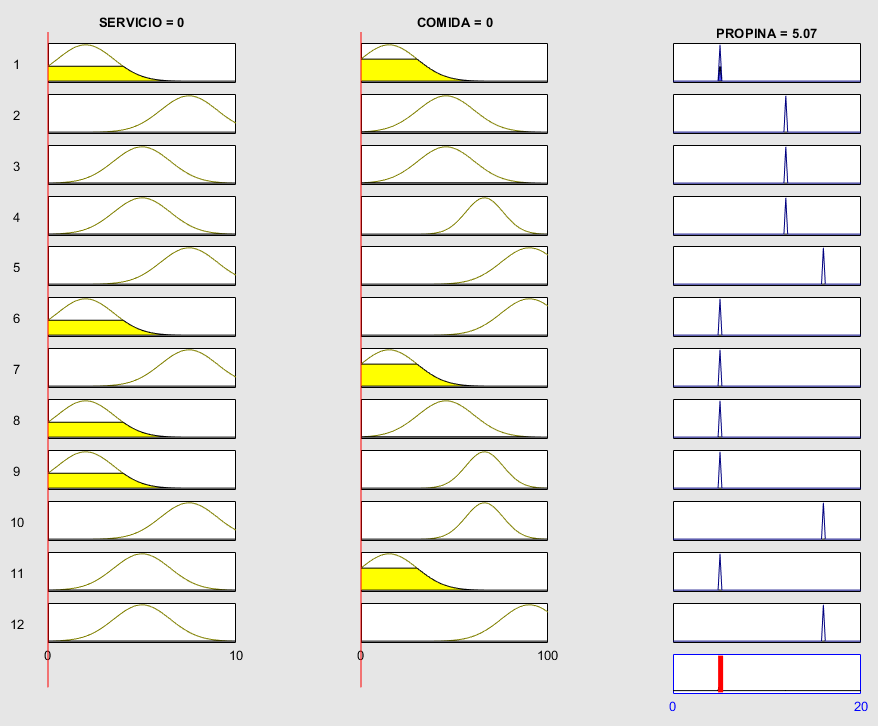
\includegraphics[width=1.4\textwidth]{IMG/RP11.png}
		\label{fig:G3}
	\end{subfigure}
	\hfill
	\begin{subfigure}{0.42\textwidth} % Reducido de 0.45
		\centering
		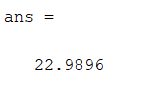
\includegraphics[width=0.4\textwidth]{IMG/M11.png}
		\label{fig:G4}
	\end{subfigure}
	\label{fig:comparacion2}
\end{figure}

A la izquierda se muestran los resultados del toolbox y a la derecha el resultado del sistema programado paso a paso. El toolbox reporta un valor de 0 para el caso planteado, mientras que el sistema programado paso a paso muestra un valor de 0. La diferencia entre ambos casos es nula, por lo que se puede afirmar que llegan al mismo resultado. Un valor de 0 en $X$ llegan a dar como resultado del seno de 0.

\newpage

\subsubsection{Caso medio}
Para el caso medio, se propone un valor de $X = 3.14$.

\begin{figure}[h]
	\centering
	\begin{subfigure}{0.40\textwidth} % Reducido de 0.45
		\centering
		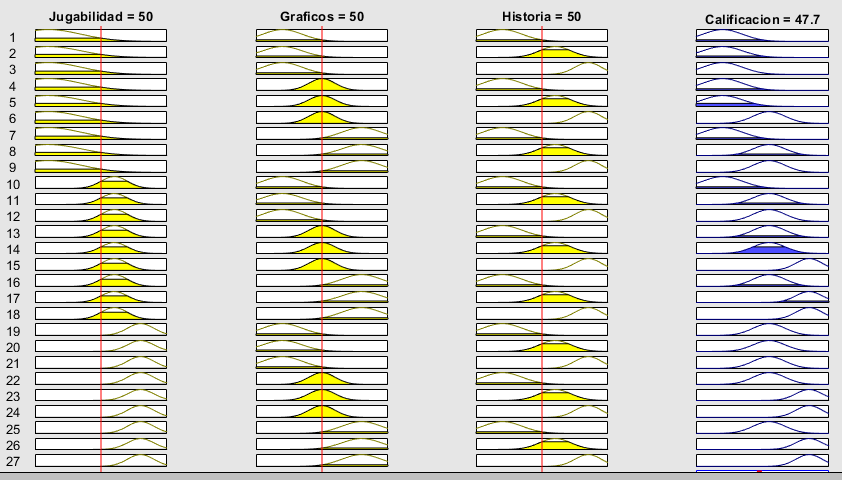
\includegraphics[width=1.4\textwidth]{IMG/RP12.png}
		\label{fig:G5}
	\end{subfigure}
	\hfill
	\begin{subfigure}{0.42\textwidth} % Reducido de 0.45
		\centering
		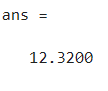
\includegraphics[width=0.4\textwidth]{IMG/M12.png}
		\label{fig:G6}
	\end{subfigure}
	\label{fig:comparacion3}
\end{figure}

A la izquierda se muestran los resultados del toolbox y a la derecha el resultado del sistema programado paso a paso. El toolbox reporta un valor de $-6.61*e^(-6)$ para el caso planteado, mientras que el sistema programado paso a paso muestra un valor de $-6.61*e^(-6)$. La diferencia entre ambos casos es nula, por lo que se puede afirmar que llegan al mismo resultado. Un valor de 3.14 en $X$ llegan a dar como resultado un seno de practicamente 0.

\newpage

\subsubsection{Caso máximo}
Para el caso máximo, se propone un valor de $X = 6.28$.

\begin{figure}[h]
	\centering
	\begin{subfigure}{0.40\textwidth} % Reducido de 0.45
		\centering
		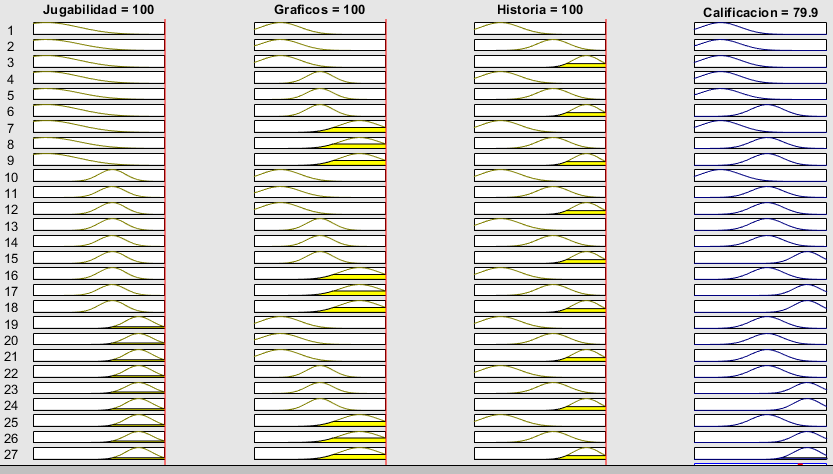
\includegraphics[width=1.4\textwidth]{IMG/RP13.png}
		\label{fig:G7}
	\end{subfigure}
	\hfill
	\begin{subfigure}{0.42\textwidth} % Reducido de 0.45
		\centering
		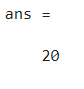
\includegraphics[width=0.4\textwidth]{IMG/M13.png}
		\label{fig:G8}
	\end{subfigure}
	\label{fig:comparacion4}
\end{figure}

A la izquierda se muestran los resultados del toolbox y a la derecha el resultado del sistema programado paso a paso. El toolbox reporta un valor de $-0.00287$ para el caso planteado, mientras que el sistema programado paso a paso muestra un valor de $-2.44*e^(-16)$. La diferencia entre ambos casos es de decimales, es relativamente pequeña, pero para efectos practicas, ambos se encuentran en casi 0, por lo que se puede afirmar que llegan al mismo resultado. Un valor de 6.28 en $X$ llegan a dar como resultado un seno de prácticamente 0.


\section{Conclusiones}

A grandes rasgos, la aproximación obtenida para la función del seno con el método de Sugeno es bastante bien acercada al comportamiento real de la función.

Se observa que no existe prácticamente diferencia entre la resolución con el toolbox y con la resolución por la implementación propia.

\newpage

\section{Referencias}

\bibliographystyle{apalike}  % Estilo de cita, puedes cambiarlo si lo prefieres.
\bibliography{Biblio}         % Aquí incluyes el archivo .bib (sin extensión).

\newpage

\section{Anexos}

Este reporte se envía con los códigos anexos que corresponden a:

\begin{enumerate}
	\item Archivo .fiz del sistema difuso para el problema de la aproximación del seno con método de Sugeno.
	\item Código en matlab para ejecutar el sistema difuso programado para el problema de la aproximación del seno con método de Sugeno.

\end{enumerate}



\end{document}

